\chapter{Introduction}
\label{sec:intro}

% Die Einleitung schreibt man zuletzt, wenn die Arbeit im Großen und
% Ganzen schon fertig ist. (Wenn man mit der Einleitung beginnt - ein
% häufiger Fehler - braucht man viel länger und wirft sie später doch
% wieder weg). Sie hat als wesentliche Aufgabe, den Kontext für die
% unterschiedlichen Klassen von Lesern herzustellen. Man muß hier die
% Leser für sich gewinnen. Das Problem, mit dem sich die Arbeit befaßt,
% sollte am Ende wenigsten in Grundzügen klar sein und dem Leser
% interessant erscheinen. Das Kapitel schließt mit einer Übersicht über
% den Rest der Arbeit. Meist braucht man mindestens 4 Seiten dafür, mehr
% als 10 Seiten liest keiner.

% \todo{adopt title page}

% \todo{adopt disclaimer}

% \todo{write introduction}

% \section{A Section}

% Referencing other chapters: \ref{sec:state} \ref{sec:design}
% \ref{sec:implementation} \ref{sec:evaluation} \ref{sec:futurework}
% \ref{sec:conclusion}

% \begin{table}[htp]
%   \centering
%   \begin{tabular}{lrr}
%     \textbf{Name} & \textbf{Y} & \textbf{Z} \\
%     \hline
%     \textit{Foo} & 20,614 & \unit[23]{\%} \\
%     \textit{Bar} & 9,914 & \unit[11]{\%} \\
%     \textit{Foo + Bar} & 30,528 & \unit[34]{\%} \\
%     \hline
%     \textit{total} & 88,215 & \unit[100]{\%} \\

%   \end{tabular}
%   \caption[Some interesting numbers]{Various very important looking numbers and sums.}
%   \label{tab:numbers}
% \end{table}

% More text referencing Table~\ref{tab:numbers}.

% \section{Another Section}

% \begin{figure}[tbp]
%   \centering
%   \includegraphics[width=0.8\textwidth]{images/squirrel}
%   \caption[Short description]{A long description of this squirrel figure.
%   Image taken from
%   \url{http://commons.wikimedia.org/wiki/File:Sciurus-vulgaris_hernandeangelis_stockholm_2008-06-04.jpg}}
%   \label{fig:squirrel}
% \end{figure}

% and Figure~\ref{fig:squirrel}.

% Something with umlauts and a year/month date:


% And some online resources:

% \section{Yet Another Section}

% \todo{add content}

% \begin{figure}[tbp]
%  \missingfigure{Come up with a mindblowing figure.}
%  \caption{A mindblowing figure}
%  \label{fig:todo}
% \end{figure}

% \section{Test commands}

% \drops \LLinux \NOVA \QEMU
% \texttt{memcpy}
% A sentence about BASIC. And a correctly formatted one about ECC\@.


% This thesis runs as follows:
% Chapter 2 State of Art
% Chapter 3 Technical Background
% Chapter 4 Design and Security Analysis
% Chapter 5 Implementation
% Chapter 6 Evaluation
% Chapter 7 Discussion

Cloud computing has become increasingly popular since it allows tenants to leverage capacity and cost advantages. As virtualization technology has matured, major vendors have introduced infrastructure as a 
service (IaaS)~\cite*{8031522}~\cite*{10.1145/2767181}.~\acrshort{IaaS} utilizes a hypervisor to manage 
virtual machines and efficiently share host resources among them. This service enables tenants to avoid peak capacity maintenance costs and promptly obtain additional compute capacity. However, VM's management, deployment, and maintenance still rely on traditional methods.
 
Consequently, the trend in cloud computing has shifted from~\acrshort{IaaS} to CaaS~\cite*{Azure_container}~\cite*{Amazon_container}~\cite*{google_container}, known as Container as a Service. Containers provide a more lightweight solution compared to virtual machines. They contain only the application and its dependencies and support automated deployment and management using a 
container orchestration platform like Kubernetes~\cite*{k8s}. Unlike virtual machines, each of which has its own operating system, containers share the host operating system, binaries, and libraries~\cite*{container_vs_vm}. As such, containers are much smaller in size than virtual machines while running at a much higher performance~\cite*{Shirinbab2020PerformanceEO}. 
Nevertheless, because containers rely on software isolation offered by the operating system, they are considered less secure than virtual machines that utilize hardware isolation mechanisms. To combine the advantages of both, the community has proposed Kata containers~\cite*{Kata-Containers}, which 
runs a group of containers within a virtual machine.
 
While Kata containers provide strong isolation at the hypervisor level for groups of containers from different tenants, it fails to ensure the confidentiality and integrity of tenants' private sensitive data. This is because the untrusted cloud provider controls the hardware and software used for 
container deployment and management. A malicious supervisor or hypervisor can access a container's secrets within a VM by inspecting the VM's memory or registers. Therefore, data privacy concerns have hindered cloud computing adoption in industries such as healthcare and finance~\cite*{data_privacy}~\cite*{eu_data_Privacy}.
 
Confidential computing proposes a mechanism that utilizes dedicated hardware to safeguard code and data on externally controlled systems. By executing the code and data within a Trusted Execution Environment (TEE) facilitated by this hardware, the code and data remain secure, even if the host system is compromised. Some examples of VM-based \acrshort{TEE}s include 
AMD SEV-SNP~\cite*{SEV_SNP_white_book}, Intel TDX~\cite*{Intel_tdx_whitepaper}, and ARM CCA~\cite*{280904}. The virtual machines running within these \acrshort{TEE}s are sometimes referred to as enclaves. The enclave's registers and memory are 
cryptographically protected, preventing access from the host operating system and hypervisor.
 
 
 
Unfortunately, these \acrshort{TEE}s are not designed to manipulate and manage containers securely. In Kubernetes~\cite*{k8s}, the responsibility for deploying and managing containers is assigned to the container runtime~\cite*{containerd}~\cite*{cri-o} on the host. It pulls the image from the image registry, launches the enclave, and coordinates the 
execution of containers in the enclave using the OCI runtime interface~\cite*{oci-runtime-spec}. Although the interface provides a way for Kubernetes to orchestrate enclaves and containers, it opens up a new attack surface. Exploiting this interface, an attacker can inject malicious code or send unauthorized commands to 
a container within an enclave. This can result in compromising the container secrets.
 
 
\begin{figure}[!htb]
  \centering
  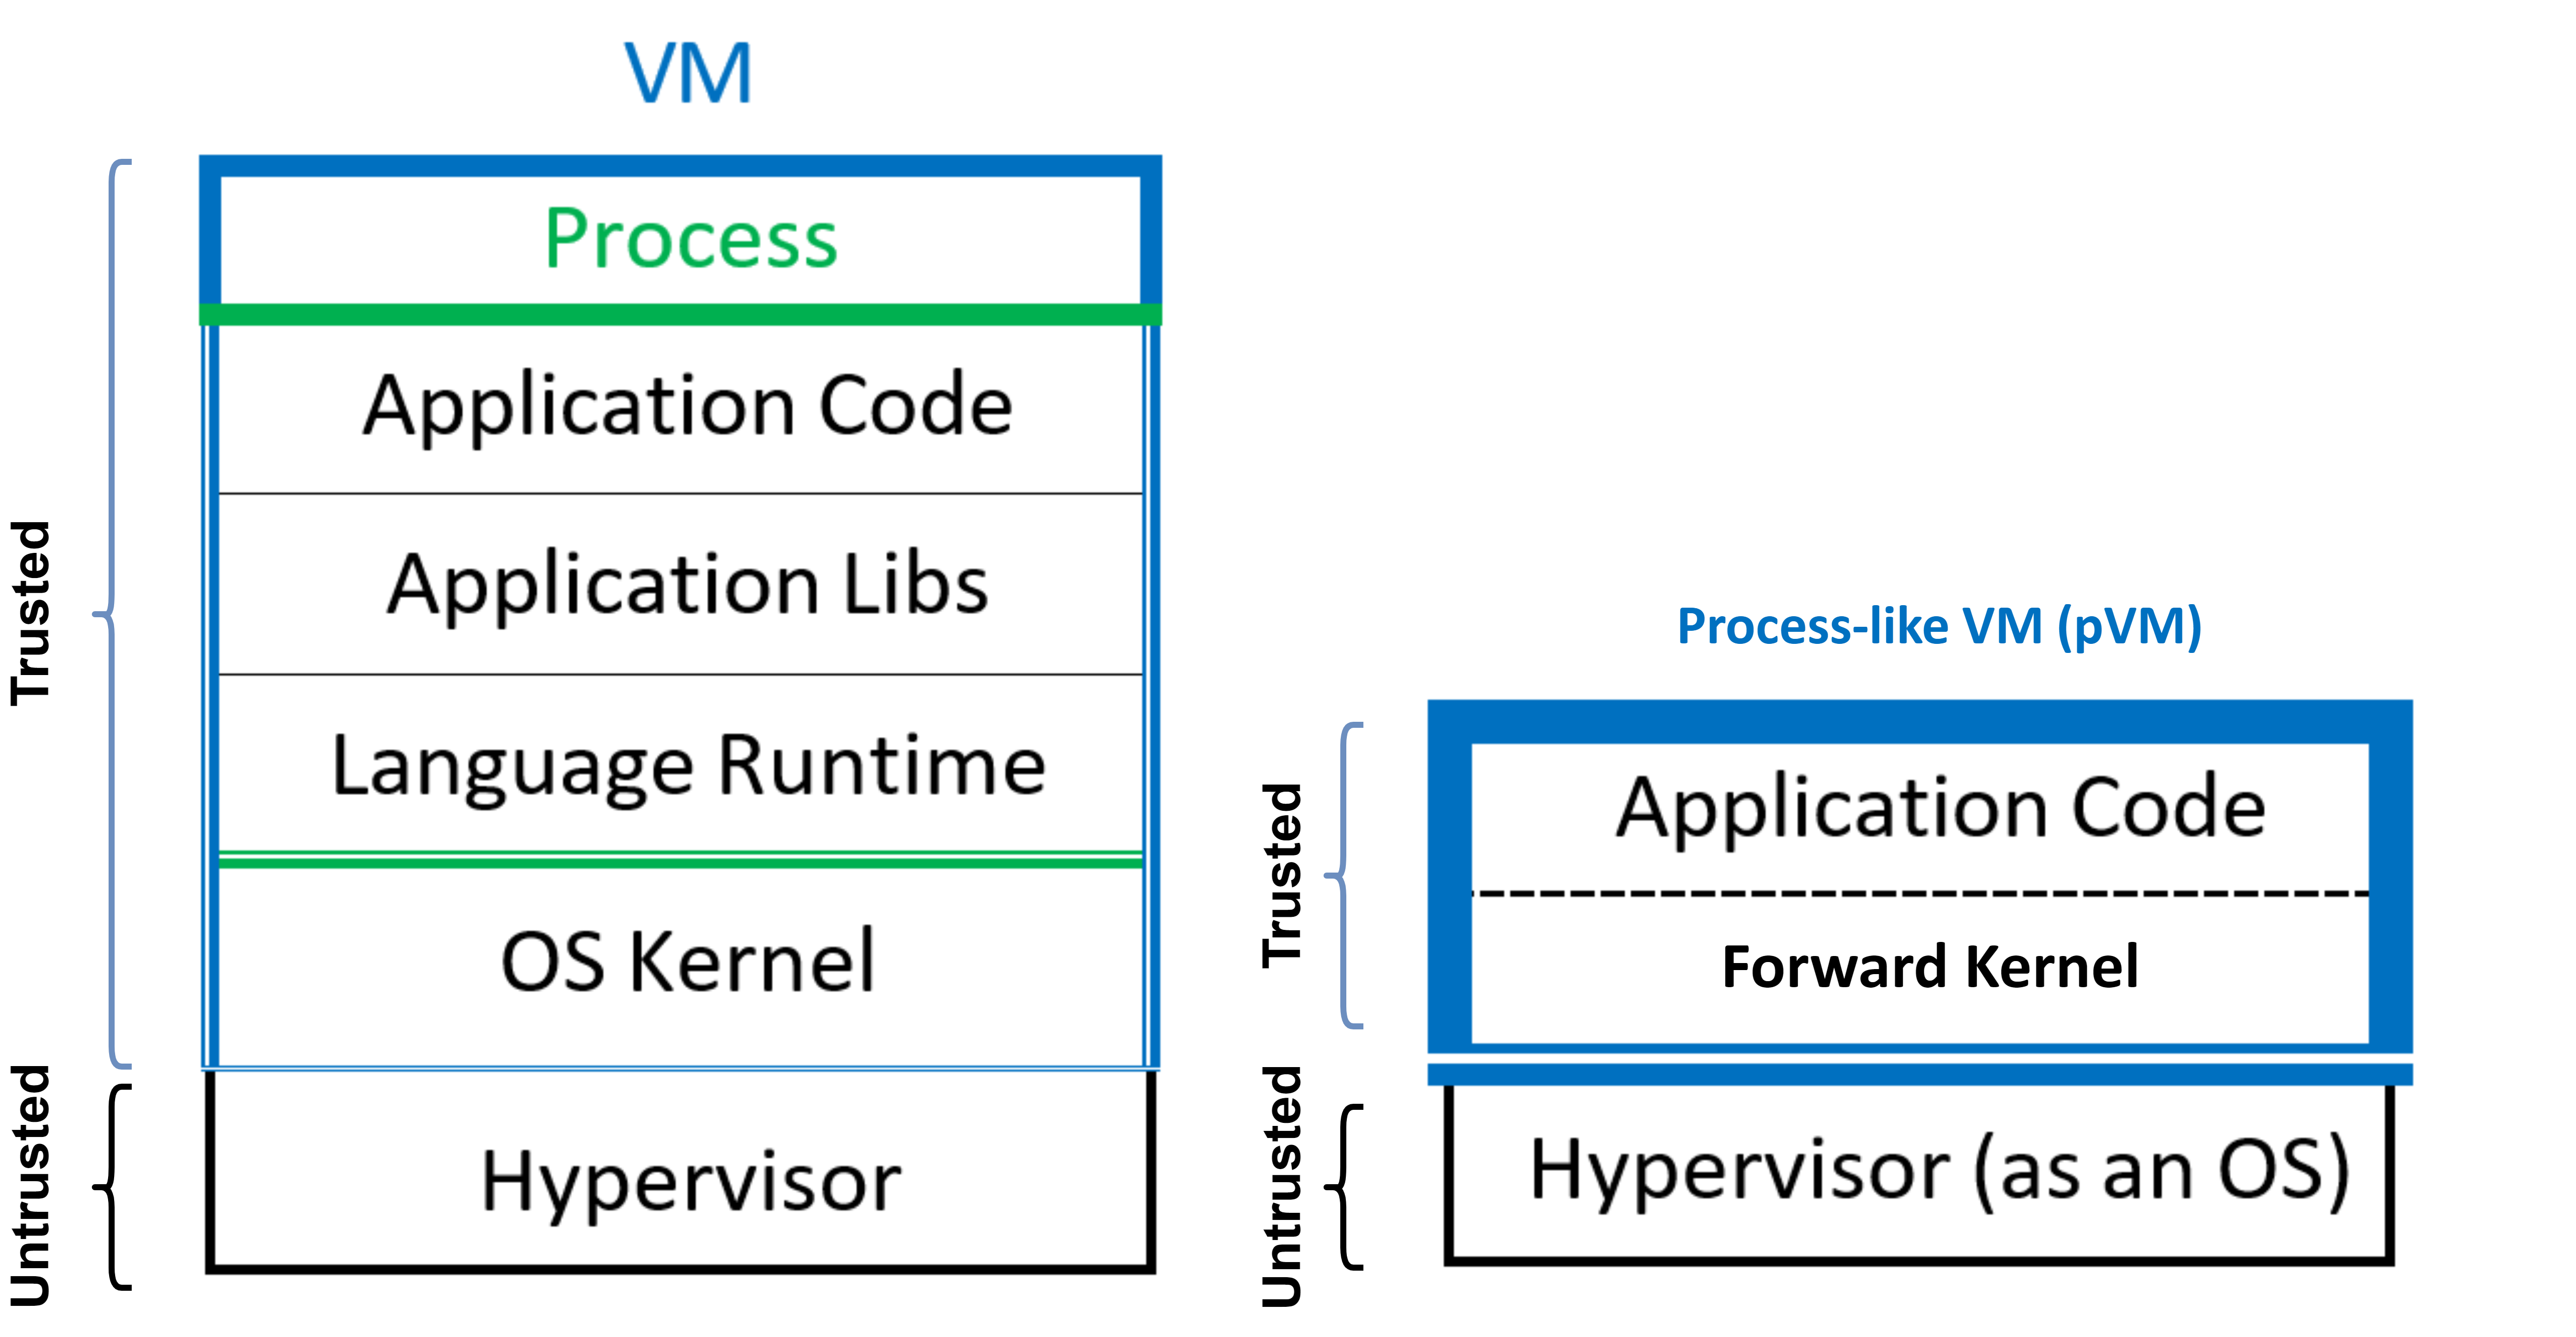
\includegraphics[width=0.6\textwidth]{images/VM_vs_PVM.png}
  \caption[Alternative virtualization architectures.]{Alternative virtualization architectures from~\cite*{10.1145/3436512}.}
  \label{fig:VM_vs_PVM}
\end{figure}
 
Another drawback of VM-based~\acrshort{TEE} is the relatively large \acrshort{TCB}. Confidential containers~\cite*{confidential_kata}, a variation of the Kata Containers in confidential computing, place a traditional KVM-QEMU VM under the protection of~\acrshort{TEE}. As depicted in Fig.~\ref{fig:VM_vs_PVM}(left), the virtual machine includes the 
user application software stack (code, libraries, language runtime (e.g., glibc~\cite*{glibc})) as well as a full OS kernel. Consequently, this amplifies the \acrshort{TCB} of the trusted execution environment, resulting in a higher potential for exploitable vulnerabilities. Hence, we consider 
the leaner approach depicted in Figure~\ref{fig:VM_vs_PVM}(right) as favorable, i.e., a process virtual machine (\acrshort{pVM}) containing only a single application and a minimized kernel. This kernel can leverage the trusted wrapper mechanisms~\cite*{Hoekstra2013UsingII} to protect the integrity and confidentiality of data within the VM and utilize services 
from the untrusted hypervisor. Using this scheme, we can effectively lower the trusted computing base of a VM and bring better performance to the application~\cite*{quark_performance_report}.
 

In order to cope with the shortcomings above, this thesis adopts Quark~\cite*{quark}, a \acrshort{pVM}-based container framework, as a foundation for investigating secure orchestration in cloud environments. By analyzing the implementation of the OCI runtime interface in Quark, we build a shielding layer within the 
enclave (\acrshort{pVM}). It enforces an enclave owner-provided policy on the OCI runtime interface. This policy ensures the confidentiality and integrity of the enclave's data and code while enabling untrusted Kubernetes to manage, deploy, and manipulate the application within the enclave as before.
 
This thesis is organized as follows:

\begin{hangparas}{.25in}{1} 

Chapter~\ref{see:art} \textit{\textbf{State of the Art}} views the work that aims to minimize the VM's TCB, then explains other mechanisms for secure orchestration in the cloud environment. 

Chapter~\ref{sec:state} \textit{\textbf{Background}} first takes a closer look at the architecture of Kubernetes\cite*{k8s} and associates open standards. It then explains the two low-level container runtimes, Kata and Quark. Next, it describes VM-based~\acrshort{TEE}, AMD SNP\cite*{SEV_SNP_white_book} and INTEL TDX~\cite*{Intel_tdx_whitepaper}. Additionally, the chapter 
introduces the KBS-attestation protocol.

Chapter~\ref{sec:security_analyse} \textit{\textbf{Security Analysis}} defines the threat model and does a secure analysis of the OCI runtime interface implemented in the Quark framework.

Chapter~\ref{sec:design} \textit{\textbf{Design}} proposes a solution for the vulnerabilities found in security analysis. It includes security deployment, a new model of EXEC, protection of process STDIO, guest log management, and guest system call interception. Finally, the chapter summarizes and generalizes the above solution and suggests changes to the OCI runtime specification.

Chapter~\ref{sec:implementation} \textit{\textbf{Implementation}} outlines how the design from the previous chapter can be implemented in the Quark framework.

Chapter~\ref{sec:evaluation} \textit{\textbf{Evaluation}} consists of qualitative and quantitative analysis. The qualitative analysis evaluates the security of our implementation. The quantitative analysis uses a set of benchmarks to assess the latency and throughput overhead imposed by our implementation.

Chapter~\ref{sec:conclusion} \textit{\textbf{Conclusion and Outlook}} summarizes our work and looks at possible future implementations.

\end{hangparas}

\cleardoublepage

